\documentclass[conference,10pt]{IEEEtran}

\usepackage{todonotes, algorithm, algpseudocode}

\begin{document}

\title{Locality-aware batch scheduling on I/O intensive workloads}

\author{Maxime GONTHIER - Carl NETTELBLAD - Elisabeth LARSSON - Samuel THIBAULT - Loris MARCHAL}
%~ \textit{LaBRI, LIP, Inria \& ENS-Lyon} \\
%~ \url{maxime.gonthier@ens-lyon.fr}}
%~ \and
%~ \IEEEauthorblockN{Loris Marchal}
%~ \IEEEauthorblockA{\textit{LIP, CNRS, ENS-Lyon, Inria} \\
%~ \url{loris.marchal@ens-lyon.fr}}
%~ \and
%~ \IEEEauthorblockN{Samuel Thibault}
%~ \IEEEauthorblockA{\textit{LaBRI, CNRS, Inria \& Univ. Bordeaux} \\
%~ \url{samuel.thibault@u-bordeaux.fr}}}

\maketitle

\begin{abstract}

\end{abstract}

\todo[inline]{Maxime: Do not hesitate to add a lot of todo notes.}

\section{Introduction}\label{sec.introduction}

\section{Related Work}\label{sec.related_work}

\paragraph{Scheduling jobs on large clusters}

To schedule jobs on batch systems, two systems are prominent: SLURM and OAR. \todo[inline]{do some research on OAR.}
SLURM is used on most HPC clusters; It's default strartegy to schedule jobs is 
First-Come First-Serve with conservative backfilling~\url{https://slurm.schedmd.com/sched_config.html}.


%~ SLURM~\cite{SLURM} is a cluster resource management system, flexible, fault-tolerant and highly scalable.
%~ First, jobs are scheduled in the FCFS order. 
%~ On top of that, the Backfill algorithm is very widely used~\cite{New_Backfill}.
%~ Backfill is, most often, based on the First Come - First Served principle as well. While the scheduler is running, jobs in the queue are sorted by priority and queueing time~\cite{New_Backfill}.
%~ Then, Backfill will start immediatly all jobs that can be started and completed without delaying the planned schedule.
%~ This algorithm allows to increase the density of supercomputer ressources' use by 20\% as well as reducing the average waiting time
%~ for execution~\cite{Maui_Scheduler}.
%~ There are two types of backfills. Coservative and EASY. Conservative backfill jobs that do not delay all other jobs. EASY backfill jobs that do not delay only the first scheduled job.
%~ EASY backfill is known to be efficient and able to prevent starvation~\cite{easybf}.
%~ \textbf{Thus our main competitor will be the EASY-Backfill algorithm.}
%~ \url{https://slurm.schedmd.com/sched_config.html} : seems to be conservative backfilling only : " If the job under consideration can start immediately without impacting the expected start time of any higher priority job, then it does so. Otherwise the resources required by the job will be reserved during the job's expected execution time". D'après \url{https://plafrim-users.gitlabpages.inria.fr/doc/#hardware} PlaFRIM utilises bien SLURM.
%~ L'article 1-s2.0-S1877050915034249-main.pdf de 2015 avance aussi que du conservative backfilling est utilisé sur leurs cluster avec SLURM.
%~ \subsubsection{OAR}
%~ Grid5k : Attention a bien prendre consciences des contraintes additionnelles qui rendent tres differentes la plateforme Grid'5000 et des plateformes HPC communes: voir la usage policy pour les contraintes jour vs nuit, et bien noter l'usage tres important de la mecanique de reservation à l'avance. Les 2 impactent bcp le scheduling "batch".
%~ D'après Pierre NEYRON ils font du conservative backfilling. Par contre atention, ils ont des usgaes policy strcte (limite par jour et illimité le soir week end) qui change tout.
%~ sauf sur nancy ou c'est du fair sharing sans limite jour nuit.
%~ Usage rate sur \url{https://intranet.grid5000.fr/stats/usage_rate.html#top}

%~ By default, SLURM, used in many HPC clusters uses FCFS coupled with 
%~ a backfilling strategy. Conservative allow for a fair treatment and 
%~ gives an expected start time to each job that is guaranteed.
%~ EASY is better to avoid starvation but does not guarantee a start time.
%~ Conservative is preferred among most of the HPC clusters.
%~ Conservative is classically implemented as follow:\\
%~ \begin{figure}[H]\centering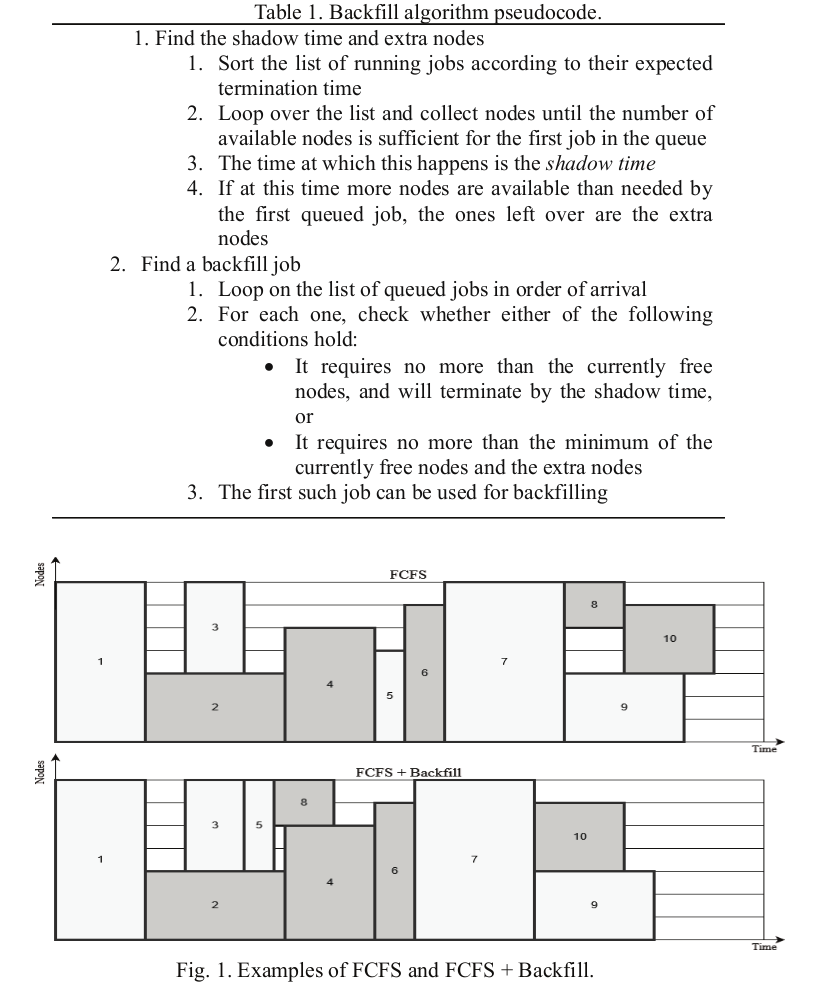
\includegraphics[scale = 0.5]{Images/conservative_backfill.png}\end{figure}

\paragraph{Ways to improve SLURM and other batch systems}

\paragraph{Memory-aware scheduling in other domains}

\paragraph{HDFS, a popular distributed file system}


%~ \subsection{Other ways to improve SLURM and other batch systems}
%~ To deal with communication-intensive jobs on SLURM, a solution is to minimize network contention by allocating nodes on the least
%~ contended switches~\cite{minimize_network_contention}. In our case we have
%~ jobs with one large file transfers that must be done before the computation start, which is different.
%~ Furthermore, we are scheduling further down the topology (i.e nodes and not switches).

%~ In "Explicit Control in a Batch-Aware Distributed File System"~\cite{Explicit_Control_in_a_Batch-Aware_Distributed_File_System},
%~ we are presented with "Batch-Aware Distributed File System", a system designed to orchestrate large, 
%~ I/O-intensive batch workloads on remote computing clusters.
%~ It adds "storage servers" that export access to the disk. And a scheduler that
%~ manage jobs. 
%~ Like us, they use detailed knowledge of workload characteristics.
%~ However, the main idea is not data reuse but to
%~ facilitates the execution of I/O intensive batch
%~ jobs by selecting appropriate storage policies
%~ in regards to I/O scoping (creating a custom environment for each job
%~ for data that will be used a lot by the job, thus not accessing the main disk too
%~ much) and space allocation.


%~ \subsection{Other papers about memory-aware scheduling}
%~ Memory-aware scheduling on clusters have been studied in the past.
 
%~ "Algorithmic Modifications to the
%~ Jacobi-Davidson Parallel Eigensolver to Dynamically Balance External CPU and Memory Load"~\cite{loadbalance_and_trashing} tackle both load balancing and memory constraint. For the load balancing, they 
%~ estimate the time needed by the fastest processor to perform the required $m$ jobs. Thus they can equilibrate the load
%~ with this information. In our study we could use a similar strategy by estimating the 
%~ processing time of a job, the length of a file transfer, and the amount of file transfers needed.
%~ To deal with memory constraint the strategy applied in the paper is to check if 
%~ nodes are thrashing data. If yes, it will recede execution of jobs on this node.
%~ The main differences are that they are using dynamic jobs. Also, we would like to 
%~ manage eviction and optimize data reuse during the scheduling phase, instead of
%~ receding execution on nodes.

%~ Some researchers~\cite{Nikolopoulos2003AdaptiveSU}
%~ are focusing on a better utilization of idling memory together with 
%~ thrashing limitation. Our focus will be to control data loads and eviction so the
%~ processing order will naturally limits thrashing.


%~ \subsection{HDFS, a popular distributed file system}
%~ HDFS~\cite{hdfs} or Hadoop Distributed File System is a distributed file system that incorporate memory-aware scheduling.
%~ HDFS is suitable for applications that have large data sets. 
%~ "Moving Computation is Cheaper than Moving Data" is an important idea for HDFS.
%~ It will migrate a computation closer to where the data is located rather than moving the data to where
%~ the application is running.
%~ Here are our main differences with HDFS. Firstly, HDFS is made for commodity hardware, prone
%~ to more errors and breakdown, so to minimize the risk of failure, data are redundant on the nodes.
%~ In our use case, the scheduler will run on professional clusters and the main point is to load as 
%~ little data as possible. Secondly, HDFS is mainly a storage system, with metadata as transactions historic or
%~ block location. Those concept are not relevant in our use case. Thirdly, the scheduling 
%~ can have issues. A paper describe in detail some problems from MapReduce~\cite{issue_with_hdfs}, the
%~ programming language used in HFDS: the static configuration of the memory allocation, the one-task assigned buffers, the
%~ lake of concurrent task running strategy and the I/O negative impact in memory during the shuffling phase.
%~ To resolve these issues, Mammoth~\cite{Mammoth} was created. It optimize memory usage on a node depending on the hardware configuration.
%~ Our approach is different because we are not dealing with MapReduce or memory allocation.
%~ Our approach is upstream. We can only allocate jobs to nodes. Moreover, we would like to maintain
%~ equity among users  while optimizing I/O.
%~ In addition, HDFS is particularly efficient when the input data used are identical over time.
%~ In our case, one user will submit a lot of different jobs using the same data, but between users,
%~ the inputs are not the same. So HDFS would be less efficient.


%~ \subsubsection{Autres}

%~ Characterization\_of\_backfilling\_strategies\_for\_parallel\_job\_scheduling.pdf compare EASY et conservative:
%~ "We observed that conserva-
%~ tive backfilling, by providing reservations to all jobs, limits
%~ backfilling opportunities. EASY backfilling on the other
%~ hand, improves backfilling opportunities but the jobs that
%~ have difficulty backfilling (e.g wide jobs) get a reservation
%~ only when they manage to get to the head of the queue,
%~ thus resulting in significant worsening in the worst-case
%~ turnaround time."


%~ \section{What can we show in an article ?}

\section{Framework}\label{sec.framework}

\section{Schedulers}\label{sec.schedulers}

In this section, we present the various schedulers used to solve
the partitioning problem presented above. 

Some of these methods uses start or completion time as a way to
schedule each job (section~\ref{subsec.fcfs_eft}) while another compute 
a score to choose the best node (section~\ref{subsec.score}) and others
ar mixed strategy between these two (sections~\ref{subsec.mixed} and~\ref{subsec.opportunistic}).

\subsection{Our two baseline schedulers: FCFS and EFT}\label{subsec.fcfs_eft}

Under our model, a fair baseline would be a scheduler capable
of reducing file transfers while keeping the First-Come First-Serve 
principle. This scheduler is Earliest Finish Time (or EFT).
It's an enhanced version of FCFS which chooses to schedule a job
on the node with the earliest available finish time, thus considering
the time to load the file, and consequently choosing nodes where a file will
be re-used. 

\begin{algorithm}[htbp]
	\caption{Earliest Finish Time (EFT)}\label{algo.eft}
	\begin{algorithmic}[1]
		\ForEach {$J_i \in \jobset$}
			\State Schedule $J_i$ on the node with the earliest completion time.
		\EndFor
	\end{algorithmic}
\end{algorithm}

Coupled with it, we add the conservative backfilling strategy mentionned earlier:

\section{Conclusion}\label{sec.conclusion}

Some schedulers do fairness as well with slurm or advance reservation with limitations.

%~ \bibliography{ref.bib}
\end{document}
